\documentclass[11pt,a4paper]{article}
\usepackage[utf8]{inputenc}
\usepackage[T1]{fontenc}
\usepackage{lmodern}
\usepackage[margin=2.4cm]{geometry}
\usepackage{amsmath,amssymb,amsthm,bm,mathtools}
\usepackage{microtype}
\usepackage{booktabs,tabularx,array}
\usepackage{enumitem}
\usepackage{xcolor}
\usepackage{tikz}
\usetikzlibrary{arrows.meta,positioning,calc,shapes.geometric,fit,backgrounds}
\usepackage{pgfplots}
\pgfplotsset{compat=1.17}
\usepackage[most]{tcolorbox}
\usepackage{caption}
\usepackage[colorlinks=true,linkcolor=blue!50!black,urlcolor=blue!50!black,citecolor=blue!50!black]{hyperref}

\captionsetup{font=small,labelfont=bf}
\setlength{\parindent}{0pt}
\setlength{\parskip}{5pt}

% ---------- colours ----------
\definecolor{geo}{HTML}{3B5BDB}
\definecolor{mat}{HTML}{D9603B}
\definecolor{lig}{HTML}{D89A00}
\definecolor{obs}{HTML}{D9604A}

% ---------- theorem environments (amsthm + boxes) ----------
\theoremstyle{definition}
\newtheorem{definition}{Definition}[section]
\newtheorem{example}[definition]{Example}
\newtheorem{algorithm}[definition]{Algorithm}
\theoremstyle{plain}
\newtheorem{theorem}[definition]{Theorem}
\newtheorem{lemma}[definition]{Lemma}
\newtheorem{proposition}[definition]{Proposition}
\newtheorem{corollary}[definition]{Corollary}
\theoremstyle{remark}
\newtheorem*{remark}{Remark}

\tcbset{thmbox/.style={enhanced,breakable,boxrule=0.6pt,arc=2pt,left=6pt,right=6pt,top=4pt,bottom=4pt,before skip=8pt,after skip=8pt}}
\tcolorboxenvironment{definition}{thmbox,colback=orange!7!white,colframe=orange!70!black}
\tcolorboxenvironment{theorem}{thmbox,colback=red!5!white,colframe=red!60!black}
\tcolorboxenvironment{lemma}{thmbox,colback=violet!5!white,colframe=violet!60!black}
\tcolorboxenvironment{proposition}{thmbox,colback=teal!6!white,colframe=teal!60!black}
\tcolorboxenvironment{corollary}{thmbox,colback=cyan!5!white,colframe=cyan!55!black}
\tcolorboxenvironment{example}{thmbox,colback=green!5!white,colframe=green!45!black}
\tcolorboxenvironment{algorithm}{thmbox,colback=gray!8!white,colframe=black!65}

\newtcolorbox{intuition}{enhanced,breakable,colback=blue!5!white,colframe=blue!60!black,
  fonttitle=\bfseries,title=Intuition,boxrule=0.6pt,arc=2pt,
  before skip=8pt,after skip=10pt}

% ---------- helpers ----------
\newcommand{\slides}[2]{\texorpdfstring{\emph{(slides #1--#2)}}{(slides #1-#2)}}
\newcommand{\slideone}[1]{\texorpdfstring{\emph{(slide #1)}}{(slide #1)}}
\newcommand{\slide}[1]{\slideone{#1}}
\newcommand{\imgplaceholder}[3][3.6cm]{%
 \begin{figure}[!htbp]\centering
 \begin{tikzpicture}
 \node[draw=black!50,dashed,thick,minimum width=0.85\textwidth,minimum height=#1,align=center,text=black!60,fill=black!3]
   {\textbf{[ Insert image from slide #2 ]}};
 \end{tikzpicture}
 \caption{#3}\end{figure}}

\DeclareMathOperator*{\argmin}{arg\,min}
\newcommand{\R}{\mathbb{R}}
\newcommand{\Sph}{\mathbb{S}^2}
\newcommand{\x}{{\bm{x}}}
\newcommand{\n}{{\bm{n}}}
\newcommand{\wi}{{\bm{\omega}_i}}
\newcommand{\wo}{{\bm{\omega}_o}}
\newcommand{\w}{{\bm{\omega}}}
\newcommand{\fr}{f_r}
\newcommand{\Lo}{L_o}
\newcommand{\Li}{L_i}
\newcommand{\Le}{L_e}
\newcommand{\cosp}{(\n^{\mathsf T}\wi)}

\title{\bfseries Foundations of Spatial AI\\[4pt]\Large Lecture 11 --- Relightable Representations}
\author{Lecture notes (Giacomini, Di Giammarino -- Sapienza University of Rome)}
\date{October 28, 2026}

\begin{document}
\maketitle
\tableofcontents
\bigskip

%==========================================================
\section{Relightable 3D Representations \slides{1}{6}}
%==========================================================

\subsection{Recap: Neural 3D Representations \slideone{3}}

Every neural 3D representation seen so far (density fields such as NeRF and 3D Gaussian Splatting, and neural surfaces such as SDFs used in IDR) can be summarised as a function that, given a 3D point and a viewing direction, returns a colour.

\begin{definition}[Radiance-field representation]
A \emph{radiance-field representation} is a parametrised function
\[
 g_\phi(\x,\w)=\bm c\in\R^3,
\]
mapping a point $\x\in\R^3$ and a direction $\w\in\Sph$ to the colour $\bm c$ observed when looking at $\x$ from direction $\w$. Density fields (NeRF, 3DGS) and neural surfaces (SDFs, e.g.\ IDR) differ in \emph{where} they place matter, but both output $\bm c$ in this way.
\end{definition}

\subsection{Radiance Fields Bake In the Lighting \slideone{4}}

In these models the colour is the light \emph{emitted} (leaving the point) towards the camera. The question is whether the model can be rendered under a different illumination. The answer is no: the lighting under which the photos were taken is baked into $g_\phi$.

\imgplaceholder[3.4cm]{4}{Radiance fields bake in the lighting (NeRF ship, IDR cans). Take the four images of slide 4. Figure credits: Mildenhall et al., ECCV 2020 (NeRF); Yariv et al., NeurIPS 2020 (IDR).}

\begin{proposition}[No relighting from a radiance field]\label{prop:norelight}
The function $g_\phi$ has no input or parameter that represents the illumination. Hence the only image-space family it can produce is the one under the capture light; changing the light requires changing $\phi$, and nothing in $\phi$ says \emph{how}.
\end{proposition}

\begin{intuition}
Think of a photograph of a statue under a desk lamp: the bright cheek and the dark side of the nose are \emph{painted} into the photo. A radiance field stores this painted result at every point. To move the lamp you would need to know the statue's real colour (the \emph{albedo}), its shape and how shiny it is --- exactly the ingredients the field never separated.
\end{intuition}

\subsection{Goal: Relightable 3D \slideone{5}}

The goal is to start from posed images under \emph{one unknown light} and produce a model that can render novel views \emph{and} novel illuminations (relit images under ``light~1'', ``light~2'', \dots).

\imgplaceholder[3.4cm]{5}{Goal of relightable 3D: novel views, relit under light 1, relit under light 2. Take the three images of slide 5. Figure credits: Zhang et al., CVPR 2021 (PhySG).}

\imgplaceholder[3.2cm]{2}{Three renderings of the same cow under different illuminations (title slide of the topic). Take the three cows of slide 2. Figure credits: S.~Tulsiani.}

\subsection{Today's Goals \slideone{6}}
\begin{enumerate}[nosep]
 \item What a relightable model needs.
 \item Why learning it from images is ambiguous.
 \item Three ways to resolve the ambiguity: \emph{constrain the model}, \emph{capture more informative data}, \emph{learn priors from data}.
\end{enumerate}

%==========================================================
\section{What We Need: The Rendering Equation \slides{7}{9}}
%==========================================================

\begin{definition}[Rendering equation, reflection form]\label{def:render}
Let $\x$ be a point on a surface with unit normal $\n$, $\Omega$ the hemisphere of directions around $\n$, and $\wo$ the outgoing direction. The radiance leaving $\x$ towards $\wo$ is
\[
 \Lo(\x,\wo)=\int_{\Omega}\underbrace{\fr(\x,\wi,\wo)}_{\text{material}}\;\underbrace{\Li(\x,\wi)}_{\text{light}}\;\underbrace{(\n^{\mathsf T}\wi)}_{\text{geometry}}\,\mathrm d\wi .
\]
\end{definition}

The three coloured factors correspond to the three unknowns of the problem: \emph{material} ($\fr$), \emph{light} ($\Li$) and \emph{geometry} (the normal $\n$ in the cosine foreshortening term, together with the surface position $\x$).

\begin{proposition}[Relighting by swapping the light]\label{prop:swap}
If material $\fr$ and geometry $(\x,\n)$ are known, then the image under any new light $\Li^{\mathrm{new}}$ is
\[
 \Lo^{\mathrm{new}}(\x,\wo)=\int_{\Omega}\fr(\x,\wi,\wo)\,\Li^{\mathrm{new}}(\x,\wi)\,(\n^{\mathsf T}\wi)\,\mathrm d\wi .
\]
This is exact for \emph{direct} light only; indirect light (light bounced from other surfaces) depends on the scene and must be recomputed.
\end{proposition}

\begin{intuition}
The equation is a recipe with three ingredients. If you know the ingredients ``material'' and ``geometry'', then ``light'' is just a plug-in slot: pull out the old light, plug in a new one, re-evaluate the integral. The caveat is that part of the light arriving at $\x$ comes from other objects in the scene, whose own appearance changes with the new light.
\end{intuition}

\subsection{Material: How a Surface Reflects Light \slideone{8}}

\begin{definition}[BRDF]
The \emph{bidirectional reflectance distribution function} $\fr(\x,\wi,\wo)\ge 0$ tells how much of the light arriving from direction $\wi$ leaves towards $\wo$. It is a function on $\Sph\times\Sph$ (four degrees of freedom) at every surface point.
\end{definition}

A \emph{shiny} material concentrates the reflected light in a narrow lobe around the mirror direction; a \emph{rough} material spreads it widely (Figure~\ref{fig:lobes}).

\begin{figure}[!htbp]\centering
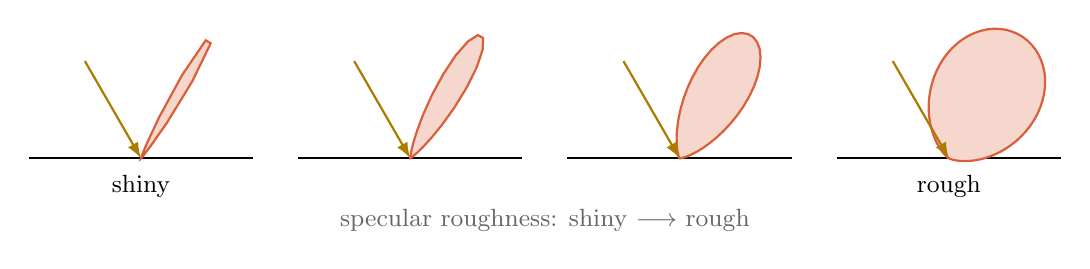
\begin{tikzpicture}[scale=0.95]
\foreach \nn/\lab [count=\i] in {200/shiny,40/{},8/{},2/rough}{
 \begin{scope}[shift={({(\i-1)*3.6},0)}]
  \draw[thick] (-1.5,0)--(1.5,0);
  \begin{scope}[rotate=-30]
   \draw[mat,thick,fill=mat!25] (0,0) -- plot[domain=-85:85,samples=70] ({1.9*pow(cos(\x),\nn)*sin(\x)},{1.9*pow(cos(\x),\nn)*cos(\x)}) -- cycle;
  \end{scope}
  \draw[lig!80!black,thick,-{Latex[length=2mm]}] ({-1.5*sin(30)},{1.5*cos(30)}) -- (0,0);
  \node[below] at (0,-0.1) {\small \lab};
 \end{scope}
}
\node[below,text=black!60] at (5.4,-0.55) {\small specular roughness: shiny $\longrightarrow$ rough};
\end{tikzpicture}
\caption{Schematic BRDF lobes for a fixed incoming direction (yellow arrow): the reflected energy (orange) is concentrated around the mirror direction for shiny materials and spreads out as roughness grows.}
\label{fig:lobes}
\end{figure}

\begin{example}[Lambertian material]
A \emph{Lambertian} (perfectly diffuse) surface has $\fr(\x,\wi,\wo)=a(\x)/\pi$, where $a(\x)\in[0,1]^3$ is the \emph{albedo}. Then
\[
 \Lo(\x,\wo)=\frac{a(\x)}{\pi}\int_\Omega \Li(\x,\wi)\,(\n^{\mathsf T}\wi)\,\mathrm d\wi=\frac{a(\x)}{\pi}E(\x),
\]
independent of $\wo$, where $E(\x)$ is the irradiance. Under constant light $\Li\equiv 1$ one has $E=\int_\Omega \cos\theta\,\mathrm d\wi=\pi$, hence $\Lo=a(\x)$: the albedo is the image of a surface under uniform unit illumination.
\end{example}

\subsection{Light: What Arrives at Each Point \slideone{9}}

The incident radiance $\Li(\x,\wi)$ is light arriving at $\x$ from \emph{every} direction of the hemisphere, and it differs at every point because of occlusion, nearby objects, etc.

\begin{figure}[!htbp]\centering
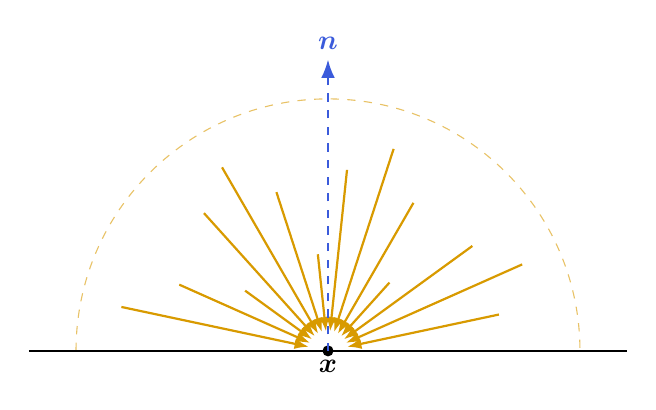
\begin{tikzpicture}
\draw[dashed,lig!60] (-3.2,0) arc (180:0:3.2);
\foreach \a in {12,24,...,168}{
 \pgfmathsetmacro{\len}{1.1+1.6*abs(sin(\a*3.7))}
 \draw[lig,thick,-{Latex[length=1.8mm]}] ({\len*cos(\a)},{\len*sin(\a)}) -- ({0.25*cos(\a)},{0.25*sin(\a)});
}
\draw[thick] (-3.8,0)--(3.8,0);
\fill (0,0) circle (2pt) node[below] {$\x$};
\draw[-Latex,geo,dashed,thick] (0,0)--(0,3.7) node[above] {$\n$};
\end{tikzpicture}
\caption{Incoming radiance $\Li(\x,\wi)$ at a surface point $\x$: one value per direction of the hemisphere (arrow length $\propto$ radiance). The normal $\n$ is dashed.}
\end{figure}

\begin{intuition}
Standing in a room, the light reaching your eye is not a single number: the window is bright, the wall opposite is dim, the ceiling in-between. $\Li(\x,\cdot)$ is a ``panorama of brightness'' seen from $\x$, and the surface multiplies it by the BRDF and sums it up. Standing under a table gives a different panorama than standing next to it.
\end{intuition}

%==========================================================
\section{Let's Learn Everything We Need \slides{10}{11}}
%==========================================================

\subsection{Learn Geometry, Material and Light with Networks \slideone{10}}

Same setup as NeRF: posed images under one unknown illumination. Each unknown is a network: an SDF network for geometry, a BRDF network for material, a light network for the light. A renderer integrates the rendering equation, and all three networks are trained jointly with a photometric loss.

\begin{figure}[!htbp]\centering
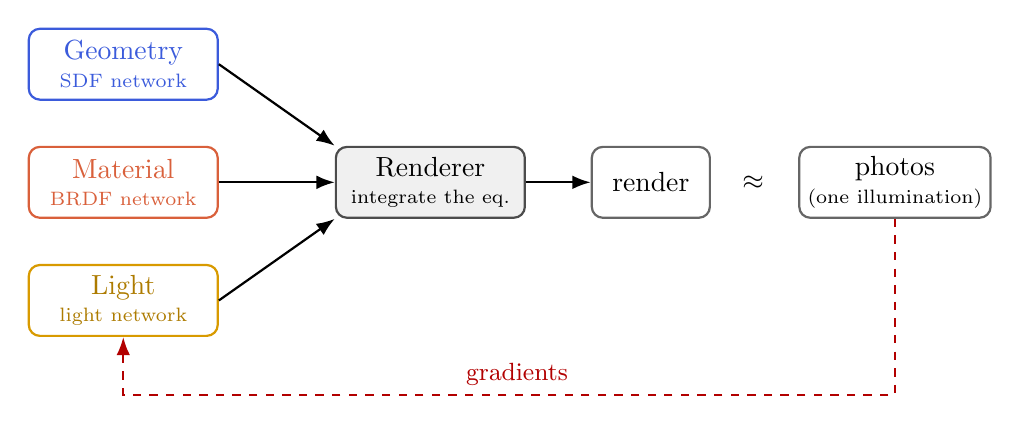
\begin{tikzpicture}[box/.style={draw,rounded corners,thick,minimum width=2.4cm,minimum height=0.9cm,align=center,inner sep=3pt}]
\node[box,draw=geo,text=geo] (G) at (0,1.5) {Geometry\\[-2pt]{\scriptsize SDF network}};
\node[box,draw=mat,text=mat] (M) at (0,0) {Material\\[-2pt]{\scriptsize BRDF network}};
\node[box,draw=lig,text=lig!80!black] (L) at (0,-1.5) {Light\\[-2pt]{\scriptsize light network}};
\node[box,fill=black!6,draw=black!70] (R) at (3.9,0) {Renderer\\[-2pt]{\scriptsize integrate the eq.}};
\node[box,draw=black!60,minimum width=1.5cm] (I) at (6.7,0) {render};
\node at (8.0,0) {$\approx$};
\node[box,draw=black!60] (P) at (9.8,0) {photos\\[-2pt]{\scriptsize (one illumination)}};
\draw[-Latex,thick] (G.east)--(R.north west);
\draw[-Latex,thick] (M.east)--(R.west);
\draw[-Latex,thick] (L.east)--(R.south west);
\draw[-Latex,thick] (R)--(I);
\draw[dashed,thick,red!70!black,-Latex] (P.south) -- (9.8,-2.7) -- (0,-2.7) -- (L.south);
\node[red!70!black,above] at (5,-2.7) {\small gradients};
\end{tikzpicture}
\caption{Inverse rendering by analysis-by-synthesis: three networks feed a differentiable renderer; the photometric error is back-propagated to all of them.}
\end{figure}

\subsection{Rendering a Pixel \slideone{11}}

The integral in Definition~\ref{def:render} is evaluated by Monte Carlo sampling.

\begin{proposition}[Monte Carlo estimator]\label{prop:mc}
Let $\wi^{(1)},\dots,\wi^{(N)}\sim p$ be i.i.d.\ directions on $\Omega$ with density $p>0$. Then
\[
 \widehat L_o(\x,\wo)=\frac1N\sum_{j=1}^N\frac{\fr(\x,\wi^{(j)},\wo)\,\Li(\x,\wi^{(j)})\,(\n^{\mathsf T}\wi^{(j)})}{p(\wi^{(j)})}
\]
is an unbiased estimator of $\Lo(\x,\wo)$.
\end{proposition}
\begin{proof}
By linearity of expectation, $\mathbb E[\widehat L_o]=\mathbb E_{\wi\sim p}\!\left[\tfrac{h(\wi)}{p(\wi)}\right]=\int_\Omega \tfrac{h}{p}\,p\,\mathrm d\wi=\int_\Omega h\,\mathrm d\wi=\Lo$, with $h=\fr\Li(\n^{\mathsf T}\wi)$.
\end{proof}

\begin{algorithm}[Rendering a pixel]
\begin{enumerate}[nosep]
 \item Find the surface point $\x$ along the pixel ray (sphere tracing on the SDF).
 \item Sample $N$ incoming directions $\wi^{(j)}\sim p$.
 \item Query the BRDF network and the light network.
 \item Average the weighted samples (Proposition~\ref{prop:mc}), compare to the photo, back-propagate.
\end{enumerate}
\end{algorithm}

\begin{intuition}
Instead of summing over \emph{all} directions (impossible), poll $N$ random ones, ask ``how much light comes from there and how much of it is sent to the camera?'', and average. Dividing by $p$ corrects for having sampled some directions more often than others, so the answer is right on average.
\end{intuition}

%==========================================================
\section{Does It Work? Why Not? \slides{12}{17}}
%==========================================================

\subsection{Does It Work? \slideone{12}}

On a synthetic cow, the fit (free per-pixel albedo plus a free environment map, fitted to one photo) reproduces the training view with error below $1/255$. But under a \emph{moving light} the fit is wrong: shading has been painted into the albedo.

\imgplaceholder[3.6cm]{12}{Photo (one illumination), fit, and moving light: truth vs.\ fit. Take the four cow images of slide 12. Figure credits: S.~Tulsiani.}

\begin{example}[What ``error $<1/255$'' means]
For pixel values in $[0,1]$, a maximum error of $1/255$ gives $\mathrm{MSE}\le(1/255)^2$ and $\mathrm{PSNR}=10\log_{10}(1/\mathrm{MSE})\ge 20\log_{10}255\approx 48.1$~dB: the training view is reproduced essentially perfectly, while the relit result is still wrong. Training error therefore says nothing about relighting quality.
\end{example}

\begin{proposition}[Trivial explanation: shading painted on, flat light]\label{prop:flat}
Consider a Lambertian scene and an observed image $I(\x)$ that is independent of the viewing direction. Take albedo $a'(\x)=I(\x)$ and a uniform environment $\Le\equiv 1$. Then the model reproduces every training image exactly.
\end{proposition}
\begin{proof}
By the Lambertian example, under $\Le\equiv1$ the rendered radiance equals the albedo, $\Lo=a'(\x)=I(\x)$.
\end{proof}

\subsection{Why? What One Capture Observes \slideone{13}}

Each surface point is seen under \textbf{one} light, from a \emph{few} directions. The unknowns are a full BRDF \textbf{and} all the incoming light.

\begin{figure}[!htbp]\centering
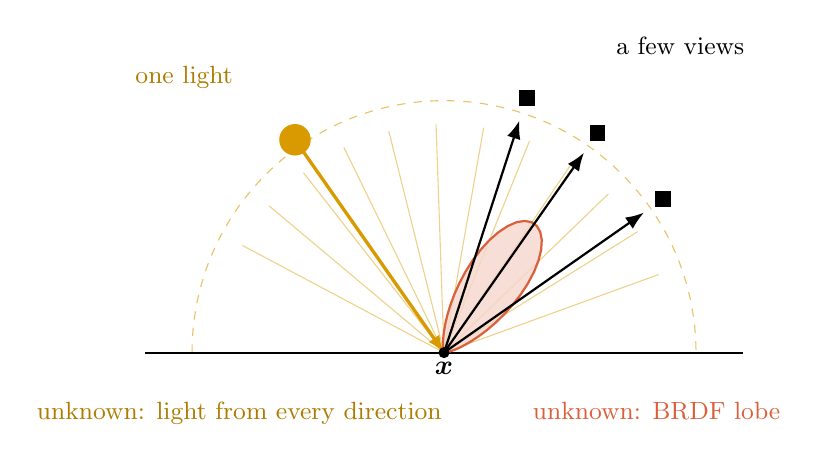
\begin{tikzpicture}
\draw[dashed,lig!60] (-3.2,0) arc (180:0:3.2);
\foreach \a in {20,32,...,160}{
 \draw[lig!45,thin] ({2.9*cos(\a)},{2.9*sin(\a)}) -- (0,0);
}
\draw[thick] (-3.8,0)--(3.8,0);
\begin{scope}[rotate=-35]
 \draw[mat,thick,fill=mat!25,fill opacity=0.8] (0,0) -- plot[domain=-70:70,samples=60] ({2.0*pow(cos(\x),10)*sin(\x)},{2.0*pow(cos(\x),10)*cos(\x)}) -- cycle;
\end{scope}
\fill[lig] ({3.3*cos(125)},{3.3*sin(125)}) circle (0.2);
\draw[lig,very thick,-{Latex[length=2.2mm]}] ({3.3*cos(125)-0.15*cos(125)},{3.3*sin(125)-0.15*sin(125)}) -- (0,0);
\foreach \a in {72,55,35}{
 \draw[-Latex,thick] (0,0) -- ({3.1*cos(\a)},{3.1*sin(\a)});
 \fill ({3.4*cos(\a)-0.1},{3.4*sin(\a)-0.1}) rectangle +(0.2,0.2);
}
\fill (0,0) circle (2pt) node[below] {$\x$};
\node[lig!80!black] at (-3.3,3.5) {\small one light};
\node at (3.0,3.9) {\small a few views};
\node[lig!80!black,below] at (-2.6,-0.5) {\small unknown: light from every direction};
\node[mat,below] at (2.7,-0.5) {\small unknown: BRDF lobe};
\end{tikzpicture}
\caption{What a single capture observes at $\x$: one light direction (thick yellow), a handful of view directions (black squares). The thin yellow rays and the orange lobe remain unconstrained.}
\end{figure}

\begin{proposition}[Counting unknowns]
At a surface point with $K$ views under one light, the data are $K$ colour values, whereas the unknowns include a BRDF (a function of 4 angular variables) and an incident-light function (2 angular variables). The unknowns outnumber the data by an unbounded factor, so the inverse problem is under-determined.
\end{proposition}

\subsection{Many Explanations, Same Pixels \slides{14}{16}}

\begin{proposition}[Factorisation ambiguity]\label{prop:amb}
For a Lambertian pixel $I=a\odot s$ (albedo $a$, shading/light term $s$, both in $\R^3_{>0}$) and any $c\in\R^3_{>0}$, the pair $(a\oslash c,\;c\odot s)$ produces the same pixel.
\end{proposition}
\begin{proof}
$(a\oslash c)\odot(c\odot s)=a\odot s=I$.
\end{proof}

\begin{figure}[!htbp]\centering
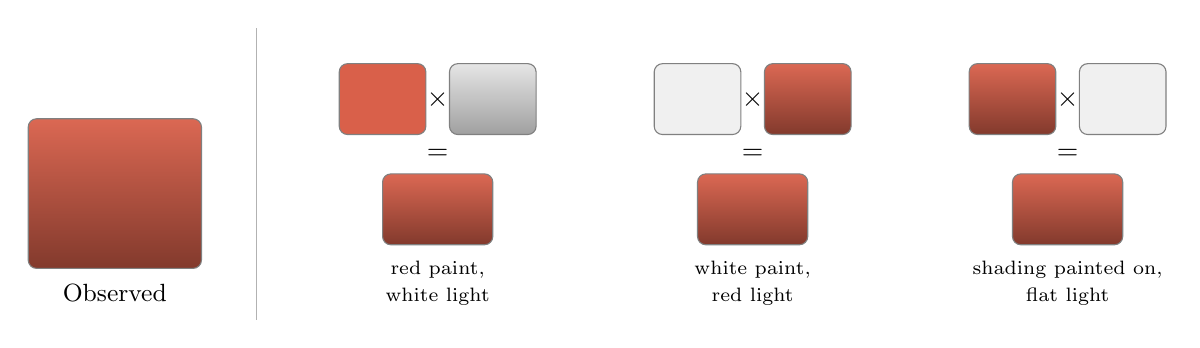
\begin{tikzpicture}[
 obj/.style={draw=black!50,rounded corners=3pt,minimum width=1.1cm,minimum height=0.9cm},
 big/.style={draw=black!50,rounded corners=3pt,minimum width=2.2cm,minimum height=1.9cm}]
\node[big,top color=obs!95,bottom color=obs!60!black] (O) at (0,0) {};
\node[below=2pt of O] {\small Observed};
\foreach \i/\albtype/\ligtype/\lab in {1/a/b/{red paint,\\white light},2/c/d/{white paint,\\red light},3/e/f/{shading painted on,\\flat light}}{
 \pgfmathsetmacro{\cx}{2.6+3.6*(\i-1)+1.0}
 \node at (\cx+0.5,1.55) {\scriptsize };
}
% explanation 1: red paint x white light
\node[obj,fill=obs] (a1) at (3.4,1.2) {};
\node at (4.1,1.2) {$\times$};
\node[obj,top color=gray!20,bottom color=gray!75] (l1) at (4.8,1.2) {};
\node at (4.1,0.5) {$=$};
\node[obj,top color=obs!95,bottom color=obs!60!black,minimum width=1.4cm] (r1) at (4.1,-0.2) {};
\node[align=center,below=2pt of r1] {\scriptsize red paint,\\[-2pt]\scriptsize white light};
% explanation 2: white paint x red light
\node[obj,fill=gray!12] (a2) at (7.4,1.2) {};
\node at (8.1,1.2) {$\times$};
\node[obj,top color=obs!95,bottom color=obs!60!black] (l2) at (8.8,1.2) {};
\node at (8.1,0.5) {$=$};
\node[obj,top color=obs!95,bottom color=obs!60!black,minimum width=1.4cm] (r2) at (8.1,-0.2) {};
\node[align=center,below=2pt of r2] {\scriptsize white paint,\\[-2pt]\scriptsize red light};
% explanation 3: shaded albedo x flat light
\node[obj,top color=obs!95,bottom color=obs!60!black] (a3) at (11.4,1.2) {};
\node at (12.1,1.2) {$\times$};
\node[obj,fill=gray!12] (l3) at (12.8,1.2) {};
\node at (12.1,0.5) {$=$};
\node[obj,top color=obs!95,bottom color=obs!60!black,minimum width=1.4cm] (r3) at (12.1,-0.2) {};
\node[align=center,below=2pt of r3] {\scriptsize shading painted on,\\[-2pt]\scriptsize flat light};
\draw[black!30] (1.8,-1.6) -- (1.8,2.1);
\end{tikzpicture}
\caption{Same pixels, many (material, light) explanations. Left: the observed shaded red object. Right: three different factorisations (albedo $\times$ light) producing it.}
\end{figure}

\begin{example}[Three explanations, one pixel]
Let the observed RGB pixel be $(0.80,\,0.35,\,0.30)$. The following all give it, channel by channel:
\begin{center}
\begin{tabular}{lcc}
\toprule
explanation & albedo $a$ & light term $s$\\
\midrule
red paint, white light & $(0.80,0.35,0.30)$ & $(1,1,1)$\\
white paint, red light & $(1,1,1)$ & $(0.80,0.35,0.30)$\\
shading painted on, flat light & per-pixel $=I$ & $(1,1,1)$ (flat)\\
\bottomrule
\end{tabular}
\end{center}
Only the first one relights correctly if the light is turned white$\to$blue.
\end{example}

\begin{intuition}
It is the same puzzle as ``is the car red, or is it white under a red light?''. A photo only records the \emph{product} albedo $\times$ light. Like trying to recover the two factors of 12 from the number 12 alone: $3\times4$, $2\times6$ and $12\times1$ are all fine, and nothing in the product tells you which one is true.
\end{intuition}

\subsection{It Happens on Real Objects \slideone{17}}

On Stanford-ORB with the \emph{same} method (nvdiffrecmc) and similar recovered shapes, the relighting PSNR of two objects is 24.4~dB versus 7.5~dB.

\begin{figure}[!htbp]\centering
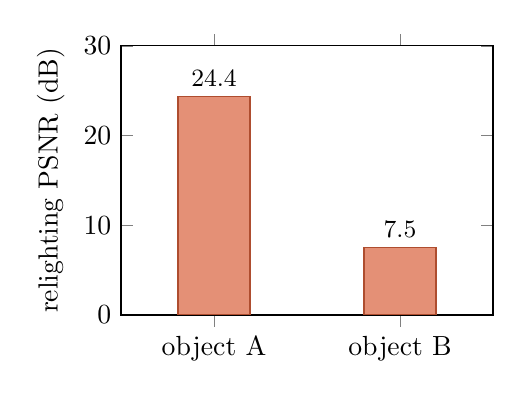
\begin{tikzpicture}
\begin{axis}[ybar,width=0.52\textwidth,height=5cm,bar width=26pt,ymin=0,ymax=30,
 symbolic x coords={object A,object B},xtick=data,ylabel={relighting PSNR (dB)},
 nodes near coords,every node near coord/.append style={font=\small},enlarge x limits=0.5]
\addplot[fill=mat!70,draw=mat!80!black] coordinates {(object A,24.4) (object B,7.5)};
\end{axis}
\end{tikzpicture}
\caption{Same method, similar shapes, very different relighting quality (values from the slide; the two objects are those of the Stanford-ORB figure).}
\end{figure}

\imgplaceholder[3.8cm]{17}{Baking and Salt objects: ground truth and prediction, novel view and relighting. Take the full 8-image grid of slide 17. Figure credits: Kuang et al., NeurIPS 2023 (Stanford-ORB).}

\begin{example}[17 dB is a lot]
Since $\mathrm{PSNR}=-10\log_{10}\mathrm{MSE}$, a gap of $24.4-7.5=16.9$~dB means a mean-squared-error ratio of $10^{1.69}\approx 49$: the relit failure is about fifty times worse in squared error, with no sign of it in the training views.
\end{example}

%==========================================================
\section{How Do We Resolve the Ambiguity? \slideone{18}}
%==========================================================

Three levers, each acting on a different part of the inverse-rendering loop:
\begin{enumerate}[nosep]
 \item \textbf{Constrain the model} (on the unknowns).
 \item \textbf{Capture more (informative) data} (on the photos).
 \item \textbf{Learn priors from data} (a learned prior over the unknowns).
\end{enumerate}

\begin{figure}[!htbp]\centering
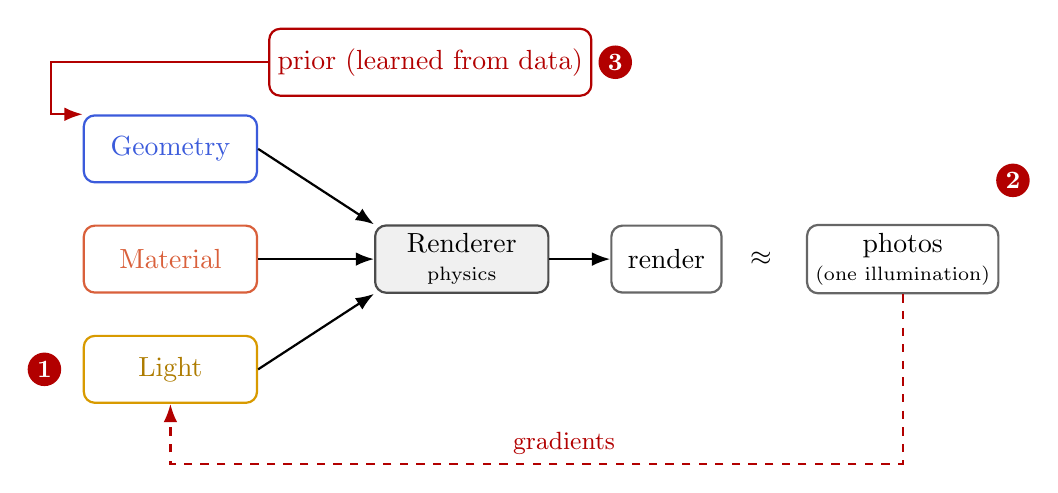
\begin{tikzpicture}[box/.style={draw,rounded corners,thick,minimum width=2.2cm,minimum height=0.85cm,align=center,inner sep=3pt},
 num/.style={circle,fill=red!70!black,text=white,inner sep=1.5pt,font=\small\bfseries}]
\node[box,draw=geo,text=geo] (G) at (0,1.4) {Geometry};
\node[box,draw=mat,text=mat] (M) at (0,0) {Material};
\node[box,draw=lig,text=lig!80!black] (L) at (0,-1.4) {Light};
\node[box,fill=black!6,draw=black!70] (R) at (3.7,0) {Renderer\\[-2pt]{\scriptsize physics}};
\node[box,draw=black!60,minimum width=1.4cm] (I) at (6.3,0) {render};
\node at (7.5,0) {$\approx$};
\node[box,draw=black!60] (P) at (9.3,0) {photos\\[-2pt]{\scriptsize (one illumination)}};
\draw[-Latex,thick] (G.east)--(R.north west);
\draw[-Latex,thick] (M.east)--(R.west);
\draw[-Latex,thick] (L.east)--(R.south west);
\draw[-Latex,thick] (R)--(I);
\draw[dashed,thick,red!70!black,-Latex] (P.south) -- (9.3,-2.6) -- (0,-2.6) -- (L.south);
\node[red!70!black,above] at (5,-2.6) {\small gradients};
\node[box,draw=red!70!black,text=red!70!black,minimum width=3.2cm] (Pr) at (3.3,2.5) {prior (learned from data)};
\draw[-Latex,red!70!black,thick] (Pr.west) -| ([xshift=-0.4cm]G.north west) -- (G.north west);
\node[num] at (-1.6,-1.4) {1};
\node[num] at (10.7,1.0) {2};
\node[num,right=2pt of Pr] {3};
\end{tikzpicture}
\caption{The three strategies: \textbf{1}~constrain what the unknowns can be, \textbf{2}~capture photos that carry more information, \textbf{3}~inject a prior learned from data.}
\end{figure}

%==========================================================
\section{Option 1: Constrain the Model \slides{19}{34}}
%==========================================================

\subsection{Constrain the Light \slideone{20}}

\begin{definition}[Distant (environment) light]
Light is \emph{far away} if it depends only on direction, not on position:
\[
 \Li(\x,\w)\approx\Le(\w)\qquad\forall\x,
\]
where $\Le:\Sph\to\R^3_{\ge0}$ is an \emph{environment map}, one per scene. Often it is additionally taken to have \emph{no colour} (a gray environment map, as in NeRS).
\end{definition}

A gray environment map removes the colour ambiguity that the NeRS paper states as ``to avoid the fundamental ambiguity (a red car vs.\ a white car under red light)'': it rules out explanation~2 of the previous section (white paint, red light).

\begin{proposition}
Under a colourless light $\Le=\ell(\w)\,(1,1,1)^{\mathsf T}$, the factorisation of Proposition~\ref{prop:amb} is restricted to scalar $c\in\R_{>0}$, so the chromatic part of the pixel colour is unambiguously assigned to albedo.
\end{proposition}
\begin{proof}
Colourless light means $s=\sigma\,(1,1,1)^{\mathsf T}$ for a scalar $\sigma$; the transformed pair $c\odot s$ stays colourless only if $c$ has equal entries. The ratios between colour channels of $a\odot s$ are then those of $a$.
\end{proof}

\imgplaceholder[3.8cm]{20}{Twelve panoramic environment maps (one per scene). Take the 4$\times$3 grid of slide 20. Figure credits: Zhang et al., NeurIPS 2021 (NeRS); Poly Haven (env maps).}

\subsection{Constrain the Material \slideone{21}}

\begin{definition}[Diffuse + specular BRDF]
\[
 \fr(\x,\wi,\wo)=\underbrace{\frac{a(\x)}{\pi}}_{\text{diffuse: varies over the surface}}+\underbrace{f_s(\wi,\wo;\rho)}_{\text{specular: few params, often shared}},
\]
with $\rho$ the specular roughness (shiny $\to$ rough, see Figure~\ref{fig:lobes}).
\end{definition}

The albedo (texture) still varies from point to point, but the specular part is often a single material for the whole object. In parameter count, a free BRDF per point has four angular variables of freedom; the constrained model has one albedo (3 numbers) per point plus one shared roughness.

\begin{intuition}
Most real objects are ``a coloured paint plus one kind of gloss''. By committing to this, we replace an infinite-dimensional unknown at every point by a handful of numbers, which the few available views can actually pin down.
\end{intuition}

\subsection{Constraints Help Even with Sparse Views \slides{22}{23}}

A constrained BRDF generalises; free-form appearance overfits. In NeRS (cars from a few images) the constrained model gives a clean result, while a version with a free radiance field, IDR and NeRF degrade.

\imgplaceholder[4.6cm]{22}{Sparse-view reconstruction: input image, NeRS, NeRS with radiance field, IDR, NeRF (two cars). Take the image grid of slide 22. Video credits: Zhang et al., NeurIPS 2021 (NeRS).}

\imgplaceholder[4.6cm]{23}{NeRS: photo, gray-albedo estimated light, and estimated environment map (three cars). Take the 3$\times$3 grid of slide 23. Figure credits: Zhang et al., NeurIPS 2021 (NeRS), Fig.~10.}

\subsection{PhySG: The Full Pipeline \slideone{24}}

PhySG instantiates all of the above in one model:
\begin{center}
\begin{tabular}{ll}
\toprule
\textcolor{geo}{Geometry} & SDF network, sphere tracing (as in lecture 09)\\
\textcolor{mat}{Material} & albedo network + \textbf{one} shared specular lobe\\
\textcolor{lig!80!black}{Light} & env map $=128$ spherical Gaussians\\
Integral & closed form (below); no shadows\\
\bottomrule
\end{tabular}
\end{center}

\subsection{Spherical Gaussians Make the Integral Closed-Form \slideone{25}}

\begin{definition}[Spherical Gaussian]
A \emph{spherical Gaussian} (SG) with axis $\bm\xi\in\Sph$, sharpness $\lambda>0$ and amplitude $\bm\mu\in\R^3_{\ge0}$ is
\[
 G(\w)=\bm\mu\,e^{\lambda(\bm\xi^{\mathsf T}\w-1)} .
\]
An environment map is approximated by a sum of SG lobes.
\end{definition}

\begin{figure}[!htbp]\centering
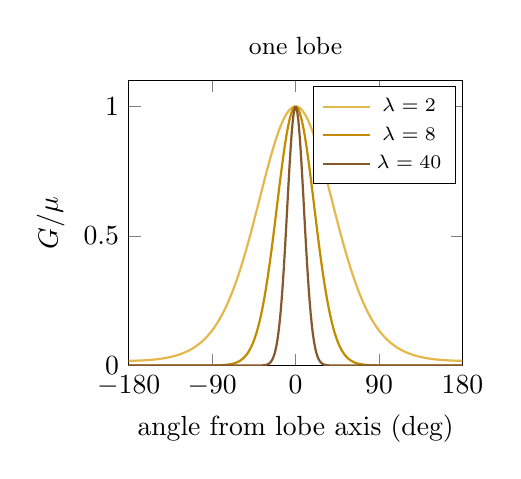
\begin{tikzpicture}
\begin{axis}[width=0.48\textwidth,height=5.2cm,xlabel={angle from lobe axis (deg)},ylabel={$G/\mu$},xmin=-180,xmax=180,xtick={-180,-90,0,90,180},ymin=0,ymax=1.1,
 legend style={font=\scriptsize,at={(0.98,0.98)},anchor=north east},title={\small one lobe}]
\addplot[domain=-180:180,samples=200,thick,lig!70]{exp(2*(cos(x)-1))};\addlegendentry{$\lambda=2$}
\addplot[domain=-180:180,samples=200,thick,lig!90!black]{exp(8*(cos(x)-1))};\addlegendentry{$\lambda=8$}
\addplot[domain=-180:180,samples=300,thick,brown!70!black]{exp(40*(cos(x)-1))};\addlegendentry{$\lambda=40$}
\end{axis}
\end{tikzpicture}\hfill
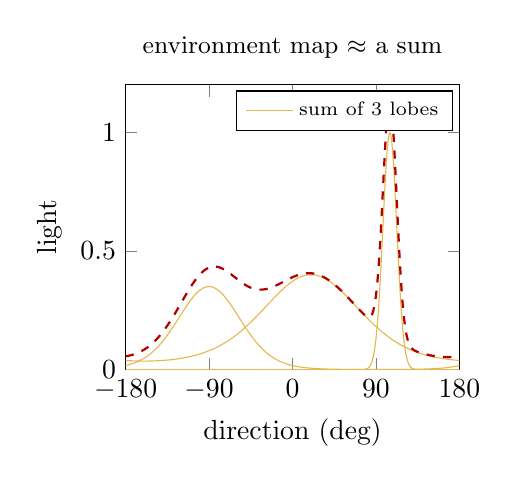
\begin{tikzpicture}
\begin{axis}[width=0.48\textwidth,height=5.2cm,xlabel={direction (deg)},ylabel={light},xmin=-180,xmax=180,xtick={-180,-90,0,90,180},ymin=0,ymax=1.2,
 legend style={font=\scriptsize,at={(0.98,0.98)},anchor=north east},title={\small environment map $\approx$ a sum}]
\addplot[domain=-180:180,samples=300,thin,lig!70]{0.35*exp(3*(cos(x+90)-1))};
\addplot[domain=-180:180,samples=300,thin,lig!70]{0.4*exp(1.2*(cos(x-20)-1))};
\addplot[domain=-180:180,samples=400,thin,lig!70]{1.0*exp(60*(cos(x-105)-1))};
\addplot[domain=-180:180,samples=400,thick,red!70!black,dashed]{0.35*exp(3*(cos(x+90)-1))+0.4*exp(1.2*(cos(x-20)-1))+1.0*exp(60*(cos(x-105)-1))};
\addlegendentry{sum of 3 lobes}
\end{axis}
\end{tikzpicture}
\caption{Left: SG lobes for increasing sharpness $\lambda$ (narrower lobe). Right: three SG lobes (thin) add up to a smooth-plus-peaked environment (dashed).}
\end{figure}

\begin{lemma}[Product of two SGs is an SG]\label{lem:prod}
For $G_k(\w)=\bm\mu_k e^{\lambda_k(\bm\xi_k^{\mathsf T}\w-1)}$, $k=1,2$, one has $G_1G_2=G_3$ with
\[
 \lambda_3=\|\lambda_1\bm\xi_1+\lambda_2\bm\xi_2\|,\quad
 \bm\xi_3=\frac{\lambda_1\bm\xi_1+\lambda_2\bm\xi_2}{\lambda_3},\quad
 \bm\mu_3=\bm\mu_1\odot\bm\mu_2\,e^{\lambda_3-\lambda_1-\lambda_2}.
\]
\end{lemma}
\begin{proof}
The exponent of the product is $\lambda_1(\bm\xi_1^{\mathsf T}\w-1)+\lambda_2(\bm\xi_2^{\mathsf T}\w-1)=(\lambda_1\bm\xi_1+\lambda_2\bm\xi_2)^{\mathsf T}\w-\lambda_1-\lambda_2=\lambda_3\bm\xi_3^{\mathsf T}\w-\lambda_1-\lambda_2=\lambda_3(\bm\xi_3^{\mathsf T}\w-1)+(\lambda_3-\lambda_1-\lambda_2)$.
\end{proof}

\begin{lemma}[Integral of an SG]\label{lem:int}
$\displaystyle\int_{\Sph}G(\w)\,\mathrm d\w=\bm\mu\,\frac{2\pi}{\lambda}\big(1-e^{-2\lambda}\big)$.
\end{lemma}
\begin{proof}
In spherical coordinates about $\bm\xi$ with $t=\cos\theta$: $\int_0^{2\pi}\!\!\int_{-1}^{1}\bm\mu\,e^{\lambda(t-1)}\,\mathrm dt\,\mathrm d\phi=2\pi\bm\mu\,e^{-\lambda}\frac{e^{\lambda}-e^{-\lambda}}{\lambda}$.
\end{proof}

\begin{theorem}[Closed-form shading with SGs]\label{thm:sg}
Let the light be $\Le=\sum_{k=1}^{K}G_k$, let the specular lobe $f_s$ be an SG in $\w$ (at fixed $\wo$ and $\n$) and let the clamped cosine be approximated by an SG $G_c$. Then
\[
 \int_\Omega \fr\,\Le\,(\n^{\mathsf T}\wi)\,\mathrm d\wi\;\approx\;\sum_{k=1}^{K}\int_{\Sph}G_k\,G_s\,G_c\,\mathrm d\w
 =\sum_{k=1}^{K}\bm\mu_k'\frac{2\pi}{\lambda_k'}\big(1-e^{-2\lambda_k'}\big),
\]
where $(\bm\mu_k',\lambda_k')$ are obtained by applying Lemma~\ref{lem:prod} twice. The cost per surface point is $O(K)$, with no sampling.
\end{theorem}
\begin{proof}
Linearity in $\Le$ turns the integral into a sum over lobes; each term is an integral of a product of three SGs, which is a single SG by Lemma~\ref{lem:prod} (applied twice), integrated by Lemma~\ref{lem:int}.
\end{proof}

\begin{intuition}
Gaussians are closed under multiplication --- the reason every Gaussian-based tool (Kalman filters, Gaussian processes) is so convenient. Here, ``light $\times$ shiny lobe $\times$ cosine'' multiplies into just one more lobe, whose total energy we know by formula. So instead of sampling hundreds of directions, PhySG evaluates $K=128$ short formulas.

Worked numbers: a lobe with $\lambda=2$ integrates to $\pi(1-e^{-4})\approx3.08\,\mu$, $\lambda=8$ to $\approx0.79\,\mu$, $\lambda=40$ to $\approx0.157\,\mu$. A lobe covers roughly $2\pi/\lambda$ steradians of the $4\pi$ sphere --- the sharper, the smaller.
\end{intuition}

\subsection{PhySG: Results \slideone{26}}

\imgplaceholder[3.8cm]{26}{PhySG: novel views, diffuse-only edit, relit under light 1 and light 2 (fish figurine). Take the four images of slide 26. Video credits: Zhang et al., CVPR 2021 (PhySG).}

\subsection{What PhySG Ignores: Shadows \& Interreflections \slideone{27}}

A shadow means less light \emph{arriving} at $\x$. PhySG's integral has no visibility term, so the only way to explain the darkness of a shadow is a darker albedo. The same holds for interreflections. The fix is shadow rays (next).

\begin{proposition}[Shadows are absorbed by albedo]\label{prop:shadow}
Let the true model be $\Lo=\frac{a}{\pi}\,V\,E$ with visibility $V\in[0,1]$ and unshadowed irradiance $E$. A model that omits $V$ fits the same pixel with albedo $a'=aV$.
\end{proposition}
\begin{proof}
$\frac{a'}{\pi}E=\frac{aV}{\pi}E=\Lo$.
\end{proof}

\begin{example}
True albedo $a=0.8$ and a point in the shadow of an occluder blocking 75\% of the light: $V=0.25$. The model without visibility reproduces the photo with $a'=0.2$. Under a new light that comes from the other side, this point would be rendered much too dark.
\end{example}

\imgplaceholder[4.2cm]{27}{Direct vs.\ indirect illumination, and albedo/roughness with and without modelling indirect illumination (hotdog scene). Take the full figure of slide 27. Figure credits: Zhang et al., CVPR 2022 (InvRender); Hasselgren et al., NeurIPS 2022.}

\subsection{Recall: Gaussians Store Baked Color \slideone{28}}

In 3D Gaussian Splatting a pixel is $\sum_i w_i\,\bm c_i(\w)$. Each Gaussian stores \emph{outgoing} light, baked in like NeRF: same problem, colour is light leaving the point.

\subsection{Relightable Gaussians (IRGS): Store Material \slideone{29}}

IRGS uses 2D Gaussians (flat disks), so each disk has a well-defined normal. Each Gaussian carries a \textbf{normal}, an \textbf{albedo} and a \textbf{roughness}; the light is one environment map, as before.

\begin{figure}[!htbp]\centering
\newcommand{\gaussians}{%
 \draw[-Latex,thick] (7.6,0)--(0.7,0);
 \draw[thick,fill=blue!35] (0.3,0) circle (0.22);
 \begin{scope}[rotate around={15:(2.6,0)}]\filldraw[fill=blue!25,draw=blue!50] (2.6,0) ellipse (0.95 and 0.3);\end{scope}
 \begin{scope}[rotate around={85:(4.6,0)}]\filldraw[fill=red!25,draw=red!50] (4.6,0) ellipse (0.8 and 0.28);\end{scope}
 \begin{scope}[rotate around={-30:(6.6,0)}]\filldraw[fill=violet!25,draw=violet!50] (6.6,0) ellipse (0.9 and 0.3);\end{scope}}
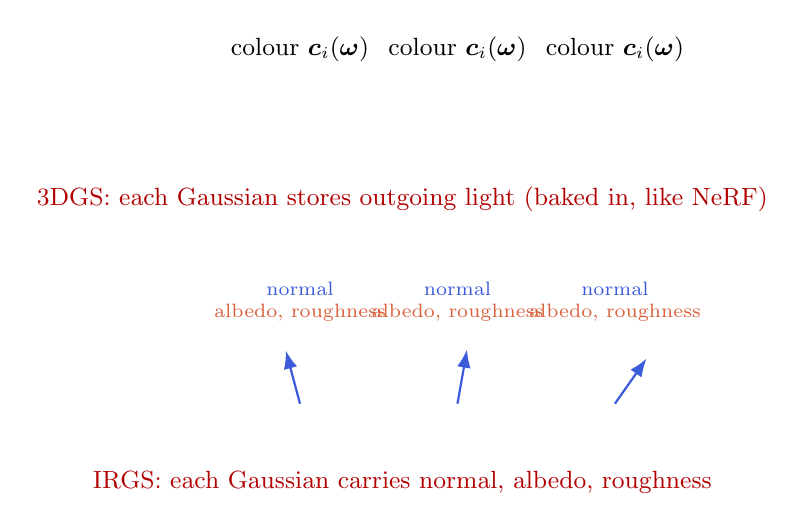
\begin{tikzpicture}
\begin{scope}
 \gaussians
 \node[align=center,font=\small] at (2.6,0.9) {colour $\bm c_i(\w)$};
 \node[align=center,font=\small] at (4.6,0.9) {colour $\bm c_i(\w)$};
 \node[align=center,font=\small] at (6.6,0.9) {colour $\bm c_i(\w)$};
 \node[red!70!black] at (3.9,-1.0) {\small 3DGS: each Gaussian stores outgoing light (baked in, like NeRF)};
\end{scope}
\begin{scope}[yshift=-3.6cm]
 \gaussians
 \foreach \xx/\ang in {2.6/105,4.6/80,6.6/55}{
  \draw[-Latex,geo,thick] (\xx,0) -- ++({0.7*cos(\ang)},{0.7*sin(\ang)});
  \node[align=center,font=\scriptsize] at (\xx,1.3) {\textcolor{geo}{normal}\\\textcolor{mat}{albedo, roughness}};
 }
 \node[red!70!black] at (3.9,-1.0) {\small IRGS: each Gaussian carries normal, albedo, roughness};
\end{scope}
\end{tikzpicture}
\caption{Top: 3DGS Gaussians store a baked colour. Bottom: IRGS Gaussians are disks with a well-defined normal and store material properties instead.}
\end{figure}

\subsection{Blend Attributes, Then Shade \slideone{30}}

\begin{definition}[Per-pixel attribute blending]
With front-to-back splatting weights $w_i$ for the Gaussians covering a pixel, the pixel receives
\[
 \bar{\n}=\sum_i w_i\,\n_i,\qquad \bar a=\sum_i w_i\,a_i,\qquad \bar r=\sum_i w_i\,r_i,\qquad \bar d=\sum_i w_i\,d_i,
\]
the blended normal (renormalised), albedo, roughness and depth $d_i$. The surface point is $\x=\bm o+\bar d\,\w$ for camera centre $\bm o$ and pixel ray direction $\w$, and the pixel colour is $\mathrm{shade}(\x,\bar{\n},\bar a,\bar r;\text{light})$.
\end{definition}

\begin{intuition}
Shading is expensive (hundreds of rays), so we do it \emph{once per pixel}, not once per Gaussian. First blend the ``G-buffer'' (normal, albedo, roughness, depth) exactly like a deferred renderer, then light the resulting surface point.
\end{intuition}

\imgplaceholder[3.2cm]{30}{Blended per-pixel attributes of the cow: normal, albedo, roughness, depth $\to\bm x$, and the shaded result. Take the five cow images of slide 30. Figure credits: Gu et al., CVPR 2025 (IRGS).}

\subsection{What About Shadows? \slideone{31}}

From $\x$ (at the blended depth), trace through the Gaussians: the accumulated opacity gives the visibility $V(\x,\w)$; and IRGS also gets \textbf{indirect light}: the colour of whatever the ray hits.

\begin{lemma}[Visibility from opacity]\label{lem:vis}
Along a ray crossing Gaussians with opacities $\alpha_1,\dots,\alpha_n$ (front to back), set $T_i=\prod_{j<i}(1-\alpha_j)$ and $w_i=\alpha_iT_i$. Then $\sum_{i=1}^{n}w_i=1-\prod_{i=1}^n(1-\alpha_i)$, so the visibility $V$ (the fraction of light that is \emph{not} absorbed) satisfies $V=1-\sum_iw_i=\prod_i(1-\alpha_i)$.
\end{lemma}
\begin{proof}
Induction on $n$. For $n=1$: $w_1=\alpha_1=1-(1-\alpha_1)$. If it holds for $n$, then $\sum_{i\le n+1}w_i=1-T_{n+1}+\alpha_{n+1}T_{n+1}=1-T_{n+1}(1-\alpha_{n+1})=1-T_{n+2}$.
\end{proof}

\begin{example}
Two Gaussians with $\alpha=(0.5,0.4)$: $w=(0.5,\;0.4\cdot0.5=0.2)$, $\sum w=0.7$, and $V=0.5\cdot0.6=0.3=1-0.7$. Only 30\% of the light gets through.
\end{example}

\begin{figure}[!htbp]\centering
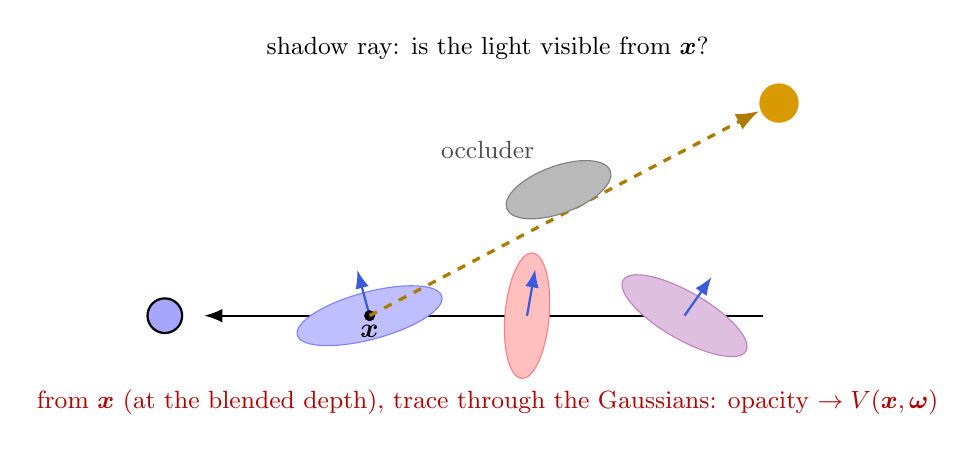
\begin{tikzpicture}
\draw[-Latex,thick] (8.0,0)--(0.9,0);
\draw[thick,fill=blue!35] (0.4,0) circle (0.22);
\begin{scope}[rotate around={15:(3.0,0)}]\filldraw[fill=blue!25,draw=blue!50] (3.0,0) ellipse (0.95 and 0.3);\end{scope}
\begin{scope}[rotate around={85:(5.0,0)}]\filldraw[fill=red!25,draw=red!50] (5.0,0) ellipse (0.8 and 0.28);\end{scope}
\begin{scope}[rotate around={-30:(7.0,0)}]\filldraw[fill=violet!25,draw=violet!50] (7.0,0) ellipse (0.9 and 0.3);\end{scope}
\foreach \xx/\ang in {3.0/105,5.0/80,7.0/55}{\draw[-Latex,geo,thick] (\xx,0) -- ++({0.6*cos(\ang)},{0.6*sin(\ang)});}
\fill (3.0,0) circle (2pt) node[below] {$\x$};
\fill[lig] (8.2,2.7) circle (0.25);
\draw[lig!80!black,dashed,very thick,-Latex] (3.0,0) -- (7.95,2.6);
\begin{scope}[rotate around={20:(5.4,1.6)}]\filldraw[fill=gray!55,draw=gray] (5.4,1.6) ellipse (0.7 and 0.3);\end{scope}
\node[gray!60!black] at (4.5,2.1) {\small occluder};
\node at (4.5,3.4) {\small shadow ray: is the light visible from $\x$?};
\node[red!70!black,align=center] at (4.5,-1.1) {\small from $\x$ (at the blended depth), trace through the Gaussians: opacity $\to V(\x,\w)$};
\end{tikzpicture}
\caption{Shadow ray from the blended surface point $\x$. If it crosses other Gaussians, their accumulated opacity reduces the visibility $V$; the colour of what it hits gives indirect light.}
\end{figure}

\subsection{Putting Shadows in the Rendering Equation \slideone{32}}

\begin{proposition}[IRGS shading estimator]
With $N$ sampled directions $\w_j\sim p$,
\[
 L_o\approx\frac1N\sum_j\fr(\w_j,\wo)\Big[\underbrace{V(\x,\w_j)}_{\text{traced opacity}}\Le(\w_j)+\underbrace{L_{\mathrm{ind}}(\x,\w_j)}_{\text{traced colour}}\Big]\frac{\n^{\mathsf T}\w_j}{p(\w_j)} .
\]
\end{proposition}

Opacity gives visibility $V$; colour gives indirect light (the Gaussians' own colour). The cost is $256$ rays per pixel, on a random subset of pixels only.

\begin{intuition}
The environment light $\Le$ is now only counted when the ray escapes ($V$ close to 1); when the ray hits something, we use that something's colour instead --- a one-bounce approximation of global illumination, implemented by the very same Gaussians. Tracing rays on just a random subset of pixels per step keeps training affordable.
\end{intuition}

\begin{algorithm}[IRGS pixel rendering]
\begin{enumerate}[nosep]
 \item Splat Gaussians: obtain blended $\bar{\n},\bar a,\bar r,\bar d$ and weights $w_i$.
 \item Compute $\x=\bm o+\bar d\w$.
 \item Sample directions $\w_j$ (256 per pixel on a random pixel subset), trace each through the Gaussians to get $V(\x,\w_j)$ and $L_{\mathrm{ind}}(\x,\w_j)$.
 \item Evaluate the BRDF from $(\bar a,\bar r)$ and sum as above; compare with the photo and back-propagate.
\end{enumerate}
\end{algorithm}

\subsection{IRGS: Results \slides{33}{34}}

\imgplaceholder[3.6cm]{33}{Global, direct and indirect illumination: the two terms of the equation rendered separately (toy scene). Take the three images of slide 33. Video credits: Gu et al., CVPR 2025 (IRGS).}

\imgplaceholder[5.0cm]{34}{IRGS materials and relighting: albedo, roughness, normal and five environment maps for four scenes. Take the 4$\times$8 grid of slide 34. Figure credits: Gu et al., CVPR 2025 (IRGS).}

%==========================================================
\section{Option 2: Capture More Informative Data \slides{35}{41}}
%==========================================================

\subsection{Capture: One Light at a Time (OLAT) \slideone{36}}

A \emph{light stage} moves a light over the sphere of directions and takes one photo per light direction (about 2048 directions in roughly a minute). Instead of one illumination, we observe each point under thousands.

\imgplaceholder[4.0cm]{36}{Light stage capture: grid of OLAT photos and the lighting environment. Take the video frame of slide 36. Video credits: Debevec et al., SIGGRAPH 2000 (Light Stage).}

\subsection{Light Adds Up \slides{37}{38}}

\begin{theorem}[Superposition of light]\label{thm:super}
For a fixed camera and scene, and linear (HDR) pixel values, let $I_A$ and $I_B$ be the images under lights $A$ and $B$ and $I_{A+B}$ the image with both on. Then $I_{A+B}=I_A+I_B$, and more generally $I(c_A A+c_B B)=c_AI_A+c_BI_B$.
\end{theorem}
\begin{proof}
The full light-transport operator (including shadows, interreflections and any number of bounces) is linear in the emitted radiance of the sources, because photons do not interact with each other: each is propagated independently and the contributions add.
\end{proof}

\begin{figure}[!htbp]\centering
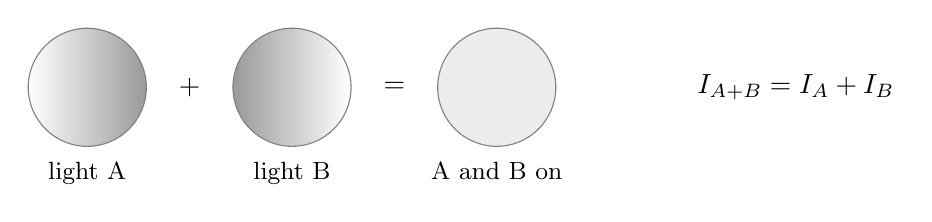
\begin{tikzpicture}
\tikzset{ball/.style={circle,draw=black!50,minimum size=1.5cm}}
\node[ball,left color=white,right color=gray!80] (A) at (0,0) {};
\node at (1.3,0) {$+$};
\node[ball,left color=gray!80,right color=white] (B) at (2.6,0) {};
\node at (3.9,0) {$=$};
\node[ball,left color=white!85!gray,middle color=white,right color=white!85!gray] (C) at (5.2,0) {};
\node[below=2pt of A] {\small light A};
\node[below=2pt of B] {\small light B};
\node[below=2pt of C] {\small A and B on};
\node at (9.0,0) {$I_{A+B}=I_A+I_B$};
\end{tikzpicture}
\caption{Light adds up: the image under two lights at once is the sum of the two single-light images (schematic sphere lit from the left, from the right, and from both).}
\end{figure}

\imgplaceholder[3.4cm]{38}{Real photos of a face under two lights and their sum. Take the video frame of slide 38. Video credits: Debevec et al., SIGGRAPH 2000 (Light Stage).}

\subsection{Light Transport Is Linear \slideone{39}}

\begin{definition}[Light-transport matrix]
Discretise the light into $K$ single-direction lights with intensities $\ell_k$ and let $I_k\in\R^{P}$ be the (vectorised) image under light $k$ alone. The \emph{light-transport matrix} is $\bm T=[I_1\,|\cdots|\,I_K]\in\R^{P\times K}$ and the image under lighting $\bm\ell$ is
\[
 I=\sum_k\ell_k I_k=\bm T\bm\ell .
\]
\end{definition}

$\bm T$ already holds material, geometry and shadows. The assumption: fixed camera and scene, linear HDR pixels.

\subsection{Relighting = a Weighted Sum \slides{40}{41}}

\begin{algorithm}[Relighting from OLAT images]
\begin{enumerate}[nosep]
 \item Capture $\{I_k\}_{k=1}^K$, one per light direction $\w_k$.
 \item For a new environment map $\Le^{\mathrm{new}}$, set $\ell_k=\Le^{\mathrm{new}}(\w_k)\,\Delta\w_k$ ($\Delta\w_k$ the solid angle of direction $k$).
 \item Output $I_{\mathrm{new}}=\sum_k\ell_kI_k$.
\end{enumerate}
\end{algorithm}

No BRDF anywhere, and no geometry: the result is just a sum.

\begin{example}
Take a pixel whose OLAT values at three lights are $(0.80,\,0.30,\,0.50)$ and a new light with weights $(0.06,\,0.90,\,0.03)$. Then $I_{\mathrm{new}}=0.048+0.270+0.015=0.333$. With $K=2048$ images of one megapixel in RGB, the table $\bm T$ holds about $2048\cdot3\cdot10^6\approx6.1\cdot10^{9}$ numbers.
\end{example}

\begin{intuition}
Imagine a dark room with 2048 tiny lamps, each lit alone for one photo. Any new lighting is a mixing board: ``a bit of lamp 17, a lot of lamp 340, \dots'' and the final photo is the same mix of the stored photos. You never needed to understand the object; the light stage did the physics for you. The price is the rig itself, and a static subject.
\end{intuition}

\imgplaceholder[4.0cm]{41}{Relighting with the light stage: weights from a captured environment map and the relit faces. Take the video frame and the strip of five faces on slide 41. Video credits: Debevec et al., SIGGRAPH 2000 (Light Stage).}

\begin{figure}[!htbp]\centering
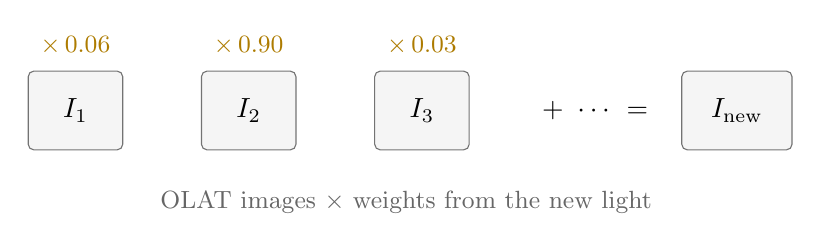
\begin{tikzpicture}[box/.style={draw=black!55,rounded corners=2pt,minimum width=1.2cm,minimum height=1.0cm,fill=black!4}]
\foreach \i/\w in {1/0.06,2/0.90,3/0.03}{
 \node[box] (b\i) at ({(\i-1)*2.2},0) {$I_{\i}$};
 \node[lig!80!black,above=2pt of b\i] {\small $\times\,\w$};
}
\node at (6.6,0) {$+\ \cdots\ =$};
\node[box,minimum width=1.4cm] at (8.4,0) {$I_{\rm new}$};
\node[below,text=black!60] at (4.2,-0.9) {\small OLAT images $\times$ weights from the new light};
\end{tikzpicture}
\caption{Relighting as a weighted sum of OLAT images (weights are those of slide 40, six out of 64 lights shown there).}
\end{figure}

%==========================================================
\section{Option 3: Learn Priors from Data \slides{42}{47}}
%==========================================================

\subsection{MaterialFusion: Prior Inside the Optimization \slideone{43}}

Keep the physical model and per-scene optimisation of Option~1, but add a learned prior on the \emph{materials}: a material diffusion model scores how plausible the rendered albedo and roughness maps are.

\begin{definition}[MaterialFusion objective]
Given posed photos under one illumination, fit mesh, materials and environment map $\theta$ by
\[
 \min_\theta\;\mathcal L_{\mathrm{photo}}(\theta)+\gamma\,\mathcal L_{\mathrm{prior}}\big(\mathrm{albedo}_\theta,\;\mathrm{roughness}_\theta\big),
\]
where $\mathcal L_{\mathrm{photo}}$ compares renders and photos, and $\mathcal L_{\mathrm{prior}}$ is a loss derived from the material diffusion model (low when the rendered albedo and roughness look like plausible materials); $\gamma>0$ sets the strength of the prior.
\end{definition}

\begin{algorithm}[MaterialFusion]
\begin{enumerate}[nosep]
 \item Input: posed photos, one illumination.
 \item Fit mesh, materials and environment map to the photos (photometric loss).
 \item Render albedo and roughness; the material diffusion model scores their plausibility $\to$ prior loss.
 \item Back-propagate the sum into $\theta$.
\end{enumerate}
\end{algorithm}

\begin{intuition}
The photo loss alone accepts any explanation that matches the pixels (the previous section's puzzle); the prior is a friend who has seen thousands of real materials and says ``a can of baking powder doesn't have a glossy sheet of random shading painted on its albedo''. In probabilistic language the prior plays the role of $-\log p(\text{materials})$ added to the data term. Priors and per-scene optimisation are not exclusive: you get both.
\end{intuition}

\imgplaceholder[3.2cm]{43}{MaterialFusion pipeline on a cow: posed photos, fitted rendering, rendered albedo and roughness. Take the images of slide 43. Figure credits: Litman et al., 3DV 2025 (MaterialFusion); S.~Tulsiani.}

\imgplaceholder[3.8cm]{44}{Relighting a real can: reference, MaterialFusion, nvdiffrecmc (same optimisation without the prior). Take the video frame of slide 44. Video credits: Litman et al., 3DV 2025 (MaterialFusion).}

\subsection{Neural Gaffer: Learn to Relight Images Directly \slideone{45}}

Neural Gaffer skips the explicit BRDF and light estimate entirely: one image plus a target environment map goes in, a relit image comes out. A diffusion model learns the mapping.

\imgplaceholder[5.0cm]{45}{Neural Gaffer: input images and relit results under environment maps and text-conditioned lights. Take the full grid of slide 45. Video credits: Jin et al., NeurIPS 2024 (Neural Gaffer).}

\subsection{How Do You Tell a Network the Light? \slideone{46}}

The environment map is converted into two images (an LDR tone-mapped copy and a log-normalised copy), both \emph{rotated into the camera frame}, VAE-encoded and concatenated with the encoded input image; the denoising U-Net (Zero123 weights, fine-tuned) produces the relit image.

\begin{figure}[!htbp]\centering
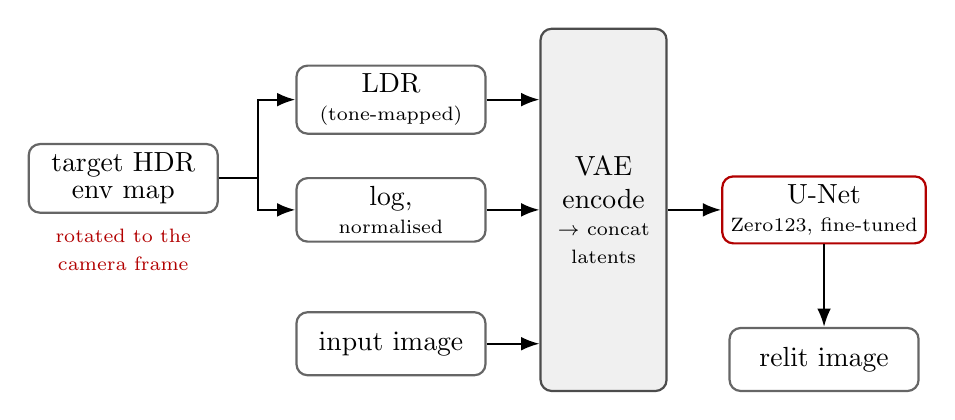
\begin{tikzpicture}[box/.style={draw,rounded corners,thick,minimum width=2.4cm,minimum height=0.8cm,align=center,inner sep=3pt}]
\node[box,draw=black!60] (E) at (0,0) {target HDR\\[-2pt]env map};
\node[red!70!black,below=2pt of E,align=center] {\scriptsize rotated to the\\[-2pt]\scriptsize camera frame};
\node[box,draw=black!60] (LDR) at (3.4,1.0) {LDR\\[-2pt]{\scriptsize (tone-mapped)}};
\node[box,draw=black!60] (LOG) at (3.4,-0.4) {log,\\[-2pt]{\scriptsize normalised}};
\node[box,draw=black!60] (IN) at (3.4,-2.1) {input image};
\node[box,fill=black!6,draw=black!70,minimum height=4.6cm,minimum width=1.6cm,align=center] (V) at (6.1,-0.4) {VAE\\encode\\[-2pt]{\scriptsize $\to$ concat}\\[-2pt]{\scriptsize latents}};
\node[box,draw=red!70!black,fill=white,minimum width=2.2cm] (U) at (8.9,-0.4) {U-Net\\[-2pt]{\scriptsize Zero123, fine-tuned}};
\node[box,draw=black!60] (O) at (8.9,-2.3) {relit image};
\draw[-Latex,thick] (E.east) -- ++(0.5,0) |- (LDR.west);
\draw[-Latex,thick] (E.east) -- ++(0.5,0) |- (LOG.west);
\draw[-Latex,thick] (LDR.east) -- (LDR.east -| V.west);
\draw[-Latex,thick] (LOG.east) -- (LOG.east -| V.west);
\draw[-Latex,thick] (IN.east) -- (IN.east -| V.west);
\draw[-Latex,thick] (V.east)--(U.west);
\draw[-Latex,thick] (U.south)--(O.north);
\end{tikzpicture}
\caption{Neural Gaffer conditioning: each env-map pixel is made to mean a fixed direction in the camera frame.}
\end{figure}

\begin{figure}[!htbp]\centering
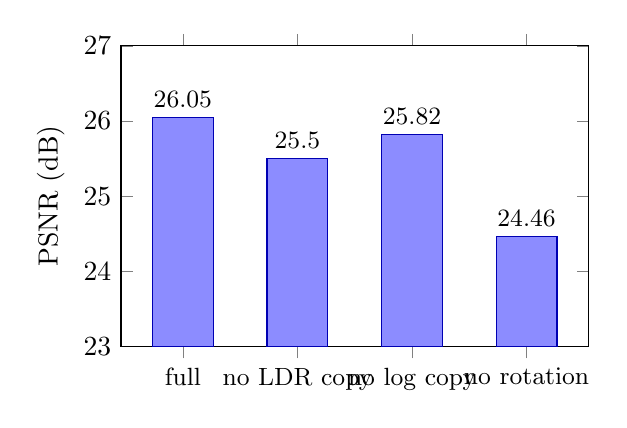
\begin{tikzpicture}
\begin{axis}[ybar,width=0.62\textwidth,height=5.4cm,bar width=22pt,ymin=23,ymax=27,
 symbolic x coords={full,no LDR copy,no log copy,no rotation},xtick=data,xticklabel style={font=\small},
 ylabel={PSNR (dB)},nodes near coords,every node near coord/.append style={font=\small},enlarge x limits=0.18]
\addplot[fill=blue!45,draw=blue!70!black] coordinates {(full,26.05) (no LDR copy,25.50) (no log copy,25.82) (no rotation,24.46)};
\end{axis}
\end{tikzpicture}
\caption{Neural Gaffer ablation (PSNR, values from the slide; the vertical axis starts at 23~dB). Removing the rotation into the camera frame hurts most ($-1.59$~dB).}
\end{figure}

\begin{intuition}
For a network, ``the light'' must be a fixed code. If the same env-map pixel meant ``north'' in one example and ``to the camera's left'' in another, the network could not learn a consistent rule; expressing the map in the camera frame gives every pixel a stable meaning, which is why dropping the rotation costs the most. The two copies help for a different reason: the LDR copy keeps the visible look, the log copy keeps the dynamic range of very bright lamps.
\end{intuition}

\subsection{Neural Gaffer: Data, 3D and Limits \slideone{47}}

\begin{itemize}[nosep]
 \item \textbf{Data:} about 90K objects and 18.4M renders, i.e.\ roughly $18.4\mathrm{M}/90\mathrm{K}\approx 200$ renders per object (many views $\times$ many lights).
 \item \textbf{3D:} relight the views, then refit the NeRF (once per target light).
 \item \textbf{Limits:} only $256^2$ images; and a yellow object or a white one under yellow light? For diffuse objects the ambiguity remains.
\end{itemize}

\imgplaceholder[4.4cm]{47}{3D relighting comparison: input views, nvdiffrecmc, TensoIR, Neural Gaffer (ours), ground truth and target lighting (three objects). Take the full grid of slide 47. Figure credits: Jin et al., NeurIPS 2024 (Neural Gaffer).}

%==========================================================
\section{Summary \slideone{48}}
%==========================================================

One illumination $\to$ many (material, light) explanations. The three remedies:
\textbf{1}~constrain the model (distant light, few-parameter BRDF, traced visibility); \textbf{2}~capture more (light is linear $\to$ relight by summing OLAT images); \textbf{3}~priors (learn plausible materials, or learn to relight directly).

\begin{table}[!htbp]
\centering\small
\renewcommand{\arraystretch}{1.25}
\begin{tabularx}{\textwidth}{>{\raggedright\arraybackslash}p{2.3cm}c>{\raggedright\arraybackslash}X>{\raggedright\arraybackslash}X>{\raggedright\arraybackslash}X>{\raggedright\arraybackslash}X}
\toprule
\textbf{Method} & \textbf{Option} & \textbf{Light / material model} & \textbf{Shadows, indirect} & \textbf{Needs} & \textbf{Main limitation}\\
\midrule
NeRF, 3DGS, IDR & -- & $g_\phi(\x,\w)=\bm c$, colour = emitted light & -- & posed images & cannot be relit: light baked in\\
NeRS & 1 & gray env map; constrained BRDF & not covered & few images of an object & light and BRDF kept simple\\
PhySG & 1 & 128-SG env map; albedo net + one shared specular lobe; SDF geometry & none (no visibility term) & posed images, one light & shadows end up in the albedo\\
IRGS & 1 & env map; per-Gaussian normal, albedo, roughness & shadow rays through Gaussians; indirect colour & posed images; 256 rays/pixel on random pixel subset & ray-tracing cost\\
Light stage (OLAT) & 2 & none: $I=\bm T\bm\ell$ & already in $\bm T$ & light-stage rig, fixed camera and scene, linear HDR & special capture setup\\
MaterialFusion & 3 & physical model + diffusion prior on albedo and roughness & via the physical renderer & posed photos, one light; per-scene optimisation & per-scene optimisation\\
Neural Gaffer & 3 & none explicit: diffusion model (image + env map $\to$ relit image) & implicit & one image + target env map; trained on ${\sim}$90K objects, 18.4M renders & only $256^2$; diffuse colour/light ambiguity\\
\bottomrule
\end{tabularx}
\caption{Comparison of the methods covered in this lecture.}
\end{table}

\begin{figure}[!htbp]\centering
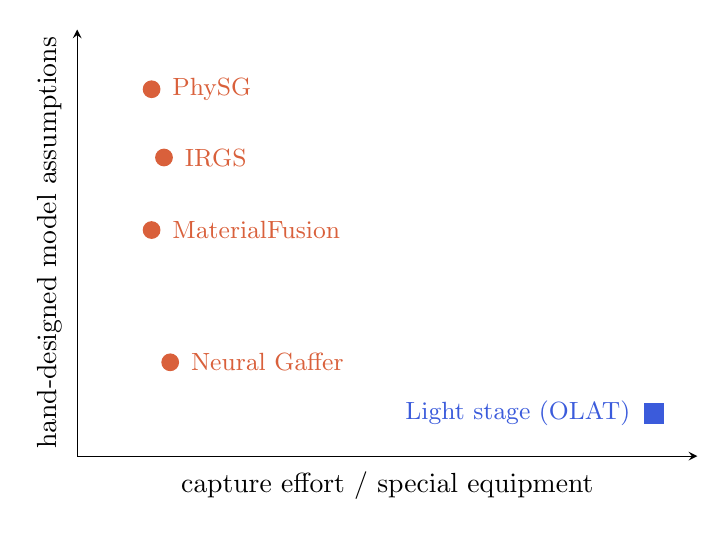
\begin{tikzpicture}
\begin{axis}[width=0.78\textwidth,height=7cm,xmin=0,xmax=10,ymin=0,ymax=10,
 xlabel={capture effort / special equipment},ylabel={hand-designed model assumptions},
 xtick=\empty,ytick=\empty,axis lines=left,
 every node near coord/.append style={font=\small}]
\addplot[only marks,mark=*,mark size=3pt,mat,nodes near coords,point meta=explicit symbolic,
 every node near coord/.append style={anchor=west,xshift=4pt,font=\small}]
 coordinates {(1.2,8.6)[PhySG] (1.4,7.0)[IRGS] (1.2,5.3)[MaterialFusion] (1.5,2.2)[Neural Gaffer]};
\addplot[only marks,mark=square*,mark size=3.5pt,geo,nodes near coords,point meta=explicit symbolic,
 every node near coord/.append style={anchor=east,xshift=-5pt,font=\small}]
 coordinates {(9.3,1.0)[Light stage (OLAT)]};
\end{axis}
\end{tikzpicture}
\caption{Schematic (qualitative, not measured) positioning of the methods: the light stage shifts the burden to the capture hardware and needs almost no model assumptions; Option~1 methods need only ordinary photos but rely on strong hand-designed assumptions; priors (Option~3) trade assumptions for learned knowledge, at the price of training data.}
\end{figure}

\subsection*{Key take-aways}
\begin{enumerate}
 \item Radiance fields store \emph{emitted} colour, so the capture lighting is baked in. Relighting needs the separate ingredients of the rendering equation: geometry, material (BRDF) and light.
 \item Fitting them from photos under one illumination is under-determined: a pixel only records the \emph{product} of albedo and light, so many (material, light) explanations fit the training views perfectly yet fail under a new light.
 \item \textbf{Constrain the model:} a distant, often colourless light, a few-parameter BRDF with a shared specular lobe, and (PhySG) spherical Gaussians for a closed-form integral; adding traced visibility and indirect light (IRGS) stops shadows from leaking into the albedo.
 \item \textbf{Capture more:} since light transport is linear, OLAT images relight by a weighted sum with no BRDF and no geometry, but it requires a special capture setup.
 \item \textbf{Learn priors:} either inside the optimisation (MaterialFusion's plausibility loss on albedo and roughness) or by learning to relight directly (Neural Gaffer), which is still limited by resolution and by the residual diffuse colour/light ambiguity.
\end{enumerate}

\bigskip
\begin{small}
\textbf{Acknowledgments.} The lecture is adapted from \emph{Learning for 3D Vision}, CMU 16-825 (Prof.\ Shubham Tulsiani). Cow illustrations by S.~Tulsiani; light-stage material from Debevec et al., SIGGRAPH 2000; results and diagrams from Mildenhall et al.\ (NeRF), Yariv et al.\ (IDR), Zhang et al.\ (PhySG, NeRS, InvRender), Kuang et al.\ (Stanford-ORB), Wang et al.\ (SIGGRAPH Asia 2009), Hasselgren et al.\ (nvdiffrecmc), Gu et al.\ (IRGS), Litman et al.\ (MaterialFusion), Jin et al.\ (Neural Gaffer); environment maps from Poly Haven.
\end{small}

\end{document}
